\documentclass[tikz,border=8pt]{standalone}
\usepackage{amsmath}
\usetikzlibrary{arrows.meta,calc,decorations.pathmorphing}
\definecolor{ink}{HTML}{21352F}
\definecolor{teal}{HTML}{087F7B}
\definecolor{blue}{HTML}{4B77A8}
\definecolor{gold}{HTML}{C58B2A}
\definecolor{rose}{HTML}{B65A62}
\begin{document}
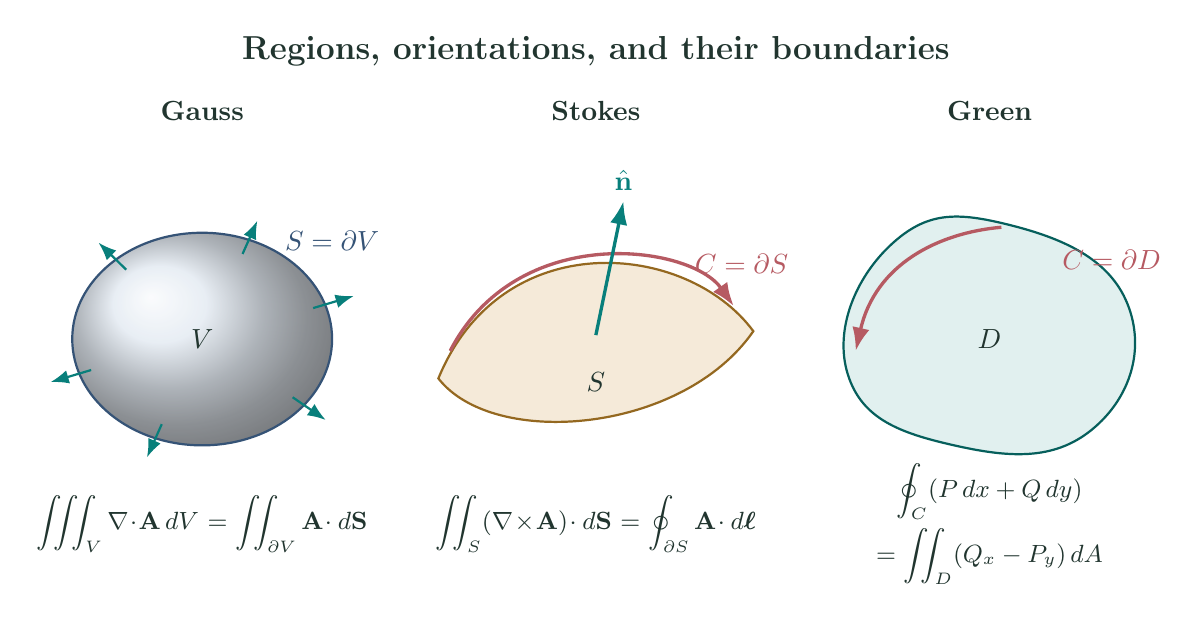
\begin{tikzpicture}[font=\sffamily,text=ink,>=Latex]
  \node[font=\bfseries\large] at (0,3.65)
    {Regions, orientations, and their boundaries};

  \begin{scope}[xshift=-5.0cm]
    \node[font=\bfseries] at (0,2.9) {Gauss};
    \shade[ball color=blue!22,opacity=.78] (0,0) ellipse (1.65 and 1.35);
    \draw[blue!70!black,thick] (0,0) ellipse (1.65 and 1.35);
    \foreach \a in {20,70,130,200,250,320}{
      \draw[teal,thick,->] ({1.5*cos(\a)},{1.15*sin(\a)})
        -- ({2.05*cos(\a)},{1.6*sin(\a)});
    }
    \node at (0,0) {$V$};
    \node[blue!70!black] at (1.65,1.25) {$S=\partial V$};
    \node[align=center,font=\small] at (0,-2.35)
      {$\displaystyle\iiint_V\nabla\!\cdot\!\mathbf A\,dV$
       $=$ $\displaystyle\iint_{\partial V}\mathbf A\!\cdot d\mathbf S$};
  \end{scope}

  \begin{scope}
    \node[font=\bfseries] at (0,2.9) {Stokes};
    \path[fill=gold!18,draw=gold!75!black,thick]
      (-2,-.5) .. controls (-1.2,1.45) and (1.15,1.25) .. (2,.1)
      .. controls (1.1,-1.2) and (-1.3,-1.4) .. cycle;
    \draw[rose,very thick,->]
      (-1.85,-.15) .. controls (-1.0,1.5) and (1.2,1.2) .. (1.75,.42);
    \draw[teal,very thick,->] (0,.05)--(.35,1.75)
      node[above] {$\hat{\mathbf n}$};
    \node at (0,-.55) {$S$};
    \node[rose] at (1.85,.95) {$C=\partial S$};
    \node[align=center,font=\small] at (0,-2.35)
      {$\displaystyle\iint_S(\nabla\!\times\!\mathbf A)\!\cdot d\mathbf S$
       $=$ $\displaystyle\oint_{\partial S}\mathbf A\!\cdot d\boldsymbol\ell$};
  \end{scope}

  \begin{scope}[xshift=5.0cm]
    \node[font=\bfseries] at (0,2.9) {Green};
    \path[fill=teal!12,draw=teal!75!black,thick]
      plot[smooth cycle,tension=.8] coordinates
      {(-1.8,-.45)(-1.25,1.2)(.25,1.45)(1.75,.45)(1.3,-1.15)(-.45,-1.35)};
    \draw[rose,very thick,->]
      (.15,1.42) .. controls (-.65,1.35) and (-1.45,.95) .. (-1.7,-.15);
    \node at (0,0) {$D$};
    \node[rose] at (1.55,1.0) {$C=\partial D$};
    \node[align=center,font=\small] at (0,-2.35)
      {$\displaystyle\oint_C(P\,dx+Q\,dy)$\\[2pt]
       $\displaystyle=\iint_D(Q_x-P_y)\,dA$};
  \end{scope}
\end{tikzpicture}
\end{document}
